\documentclass[a4paper,12pt]{article}
\usepackage[utf8]{inputenc}
\usepackage[T1]{fontenc}
\usepackage[UKenglish]{babel}
\usepackage{graphicx}
\usepackage{geometry}
\geometry{a4paper,
		     tmargin = 35mm, 
		     lmargin = 30mm,
		     rmargin = 30mm,
		     bmargin = 30mm}
\usepackage{mathtools}
\usepackage{amsmath}
\usepackage{color}
\usepackage{setspace}
\usepackage{amsmath,amssymb}
\usepackage{float}
\usepackage{hyperref}

\usepackage{indentfirst}
\usepackage{subfig}

\usepackage{siunitx}

\renewcommand\thesection{\Roman{section}.}
\renewcommand\thesubsection{\thesection\arabic{subsection}.}
\begin{document}

\linespread{1.25}

\begin{titlepage}

    \centering
    
\includegraphics[width=0.66\textwidth]{elte.jpg}\par\vspace{1cm}
    {\scshape\LARGE ELTE \par}
    \vspace{3cm}
    {\scshape\Large Astronomical observational exercises at Piszkéstető\par}
    \vspace{1cm}
    {\large\itshape György Baranka, Dénes Berta, Alex Olar\par}
    \vspace{3cm}
    {\large 2018 \par}

\end{titlepage}

\tableofcontents

\newpage

\section{Introduction}

\subsection{About Piszkéstető}

\par The observatory at Piszkéstető consists of three main telescopes
in different sizes. It is the biggest facility in Hungary that is capable of
making astronomical measurements. The observatory due to its location and the size of the telescopes
is mostly able to see brighter objects but on these long-term measurements can
be executed. Photometric and spectrographic measurements are being done during our
stay and even new CCD chips have been deployed to one of the telescopes.

\subsection{CCDs}

\par CCDs are semiconductor devices that are highly effective in capturing most of the
incoming light and converting photons to electrons. The conversion rate is called
quantum effectivity (QE) which is very high in CCDs and pretty low in digital cameras.
Not only do they work effectively but also they have linear response - called gain - which
is basically the number of resulting electrons per photon.

\subsubsection{Image pre-processing}

\par Due to the CCD architecture there are a number of pre-processing steps
to be done before anylizing an image.

\begin{enumerate}
    \item \textbf{overscan removal}: it is calculated by the CCD camera by the creation of
          extra pixels in a row, the mean value of this should be subtracted from the image and the extra row
          removed/trimmmed
    \item \textbf{de-biasing}: subtraction of the mean pixel values that are acquired as a mean of zero exposure
          images
    \item \textbf{dark noise correction}: taking images with the same exposure time with a closed shutter in order
          to be able to remove thermal noise - CCD chips are usually cooled to a low temparature, given a low enough temperature, this noise
          can be almost eliminated - this is also done by acquiring and averaging more images
    \item \textbf{flattening}: by taking images of an evenly illuminated CCD chip one can correct for the chip's individual pixel sensitivity
          and also for dust particles that are stuck to the chip as well as vignetting at the edges
\end{enumerate}


\par After having acquired the master images of bias, dark and flat we needed to substract the first two and
divide by the latter which was scaled between 0-1 by \textit{fitsh}.

\par During this lab the CCDs did not create overscan pixels so that step should have been skipped but we did that
following three steps with a software package called \textit{fitsh} \footnote{https://fitsh.net/} which is a C library
designed for the analysis and processing of CCD images.

\section{Measurements}

\subsection{Photometry analysis of XX Cyg cepheid}

\par We were given archive images of a pulsar called \textbf{XX Cyg} and we did the preprocessing steps with the above mentioned package.
After the images were pre-processed we run some scripts with \textit{fitsh} to find stars over a given pixel-threshold ($10000$) then we
used one of the measurements as reference image. This was necessary as the different images were taken in a period of time and
the field of view was rotated and shifted during the process. The last step was to transform these images into the same view.

\vspace{0.5cm}

\begin{minipage}{0.42\textwidth}
    \begin{figure}[H]
        \centering
        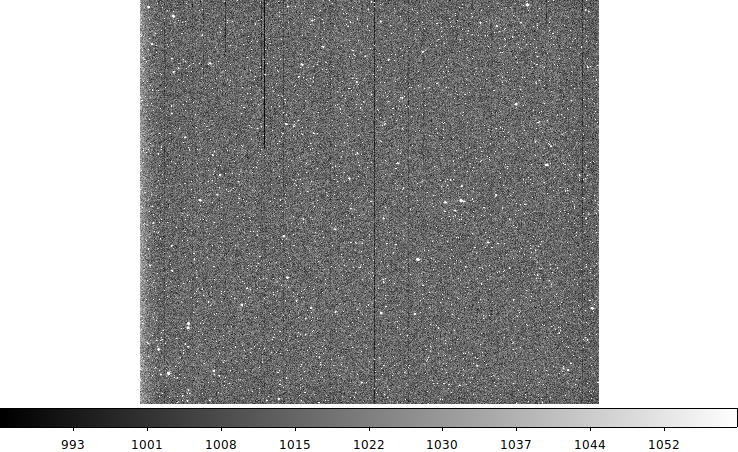
\includegraphics[width=0.9\textwidth]{../PSCH-20181012/psch/20181012/before200.png}
        \caption{Before preprocessing and transformation}
    \end{figure}
\end{minipage}
\begin{minipage}{0.42\textwidth}
    \begin{figure}[H]
        \centering
        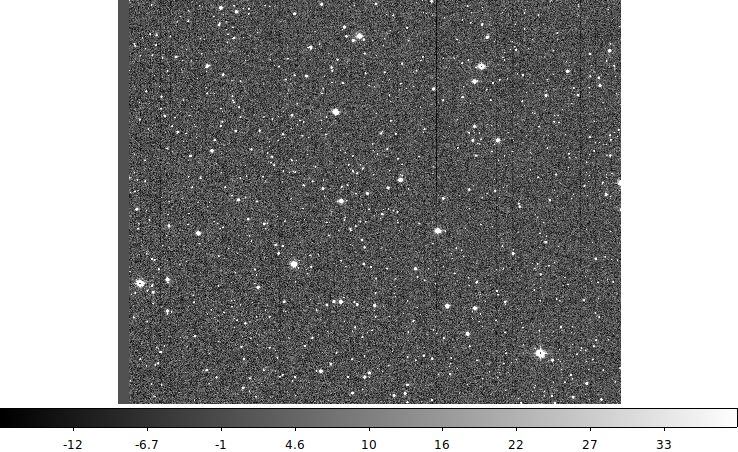
\includegraphics[width=0.9\textwidth]{../PSCH-20181012/psch/20181012/after200.png}
        \caption{After preprocessing and transformation}
    \end{figure}
\end{minipage}

\vspace{0.5cm}

\par We also had a program that visualized stars and with this we were able to select our star
and the start to that we compared it with. This can be seen in the plot below:

\begin{figure}[H]
    \centering
    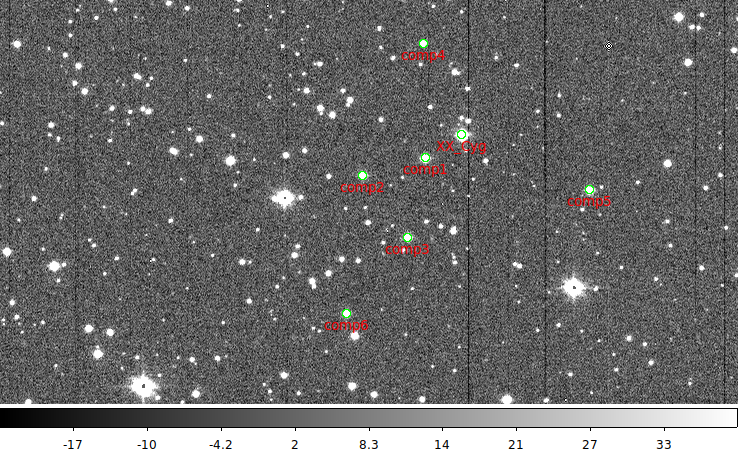
\includegraphics[width=0.75\textwidth]{../PSCH-20181012/psch/20181012/withStars.png}
    \caption{The target and comapring stars (XX Cyg and comp1-6)}
    \label{fig:jd}
\end{figure}

\par We then extracted the photometric data with \textit{fitsh} and created plots
of the target and comparing magnitudes in filters R and V. The periodicity can be seen
on the image as well as that the choosen stars for comparison were good enough since 
they do not vary a lot compared to each other.

\begin{figure}[H]
    \centering
    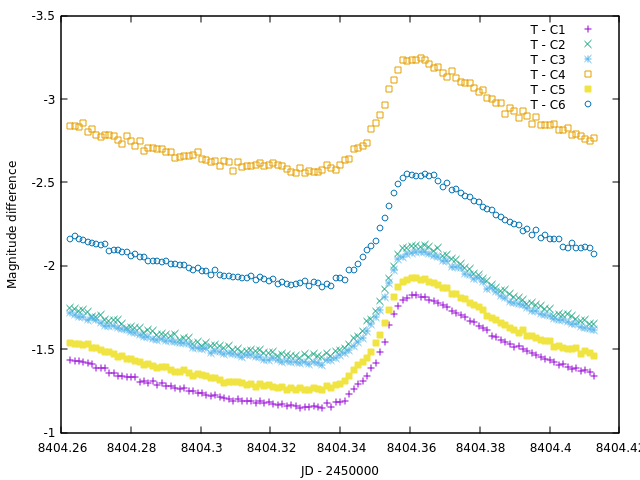
\includegraphics[width=0.75\textwidth]{../PSCH-20181012/psch/20181012/mag-jd.png}
    \caption{Magnitude difference with each comapring star given the Julian date of images}
\end{figure}

\begin{figure}[H]
    \centering
    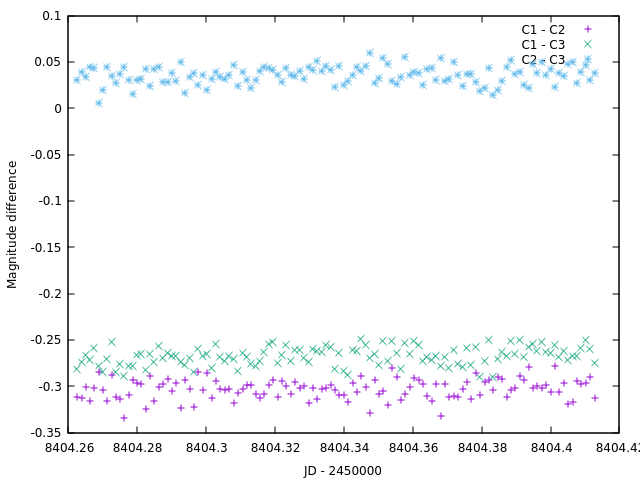
\includegraphics[width=0.75\textwidth]{../PSCH-20181012/psch/20181012/mag-jd-comp.png}
    \caption{Magnitude difference of some comparing stars given Julian date}
\end{figure}

\par These measurements were done with the Schmidt-telescope in 2018/10/12. The periodic time of
XX Cyg is approximately $3~h$ and $14~min$ which is $\approx 0.14$ JD. Given \ref{fig:jd} it can be seen that the frame
is $0.16$ JD and it seemingly shows around 1 period.

\subsection{RGB image from RC-80 image filters}

\par We also got images taken on 2019/02/06 on which we did the preprocessing steps and used the
r, g, B filters on images of galaxy M51. We then uploaded these images to a site \footnote{http://nova.astrometry.net/upload}
in order to fill the header files with the appropriate celestial coordinates. These were needed for the
python $aplpy$ package which used $astropy$ to correctly make an RGB image from the corrected r, g, B 
filters. After hours of unsuccessful tries we finally were able to create a pretty RGB image 
of the galaxy.

\vspace{0.6cm}

\begin{figure}[H]
    \centering
    \includegraphics[width=0.95\textwidth]{../rc80/2019-02-06/reg/bestMaster.png}
    \caption{RGB image of galaxy M51}
\end{figure}

\newpage

\section{Conclusion}

\par We had a nice weekend at Piszkéstető. We got acquainted with the
experiments that are being done here and also we were shown how to process
and analyse images on our own. Róbert was very helpful and patient with us
and everything went smoothly during our stay. We uploaded our scripts to GitHub 
\footnote{Our scripts: https://github.com/qbeer/piszkesteto}.

\end{document}
